\documentclass[12pt]{article}
\usepackage{a4,fancyhdr,moreverb,epsfig,amssymb,amsmath,ifthen}
\usepackage[utf8]{inputenc}
\usepackage[english]{babel}
\usepackage{mathtools}
\usepackage{lstautogobble}
\usepackage[framed,numbered]{mcode}
\usepackage{listings}
\usepackage{amsthm}
\textwidth 455pt \oddsidemargin 0mm
\parindent 12pt
\textheight 685pt % old : 665pt
\textheight 697pt
\topmargin -40pt  % old -70pt
\newcommand{\cpp}{C\raisebox{.4ex}{\tiny ++}}
\renewcommand{\vec}{\underline}
\newcommand{\va}{\underline{a}}
\newcommand{\vb}{\underline{b}}
\newcommand{\vc}{\underline{c}}
\newcommand{\vh}{\underline{h}}
\newcommand{\ve}{\underline{e}}
\newcommand{\vg}{\underline{g}}
\newcommand{\vp}{\underline{p}}
\newcommand{\vq}{\underline{q}}
\newcommand{\vu}{\underline{u}}
\newcommand{\vv}{\underline{v}}
\newcommand{\vw}{\underline{w}}
\newcommand{\vx}{\underline{x}}
\newcommand{\vy}{\underline{y}}
\newcommand{\vz}{\underline{z}}
\newcommand\myeq{\stackrel{\mathclap{\normalfont\mbox{cgs}}}{=}}
\newcommand{\dd}[1]{\mathrm{d}#1}


\usepackage{graphicx}
\graphicspath{ {./images/} }


\begin{document}
\pagestyle{fancyplain}
\lhead{\fancyplain{}{\sf M4S18B2 Machine Learning}}
\rhead{\fancyplain{}{\sf Omar Haque}}
\cfoot{}{}


\begin{center} \Large
Machine Learning - Coursework 1 \\[4mm]
\end{center}

\par \hfill\hrulefill\hfill \vspace{2mm}


\vspace{0.3in}

\begin{itemize}
\item \textbf{Calculate and plot the average face of the training set, then write a function to find a PCA basis of size M, where the inputs will be M and X, the matrix containing the training set. Clearly describe all aspects of your function, then use it to plot the first 5 eigenfaces of the training set.}
\end{itemize}

To calculate the average face of the training set, I simply calculate the average pixel values for each pixel across the trainings set.

\begin{lstlisting}[linewidth=18.4cm,language=R]
library(rARPACK)
library(philentropy)


# I load the raw csv's
faces.train.inputs <- read.csv("./2018_ML_Assessed_Coursework_1_Data/
                               Faces_Train_Inputs.csv",head=FALSE)
faces.train.label <- read.csv("./2018_ML_Assessed_Coursework_1_Data/
                              Faces_Train_Labels.csv",head=FALSE)
faces.test.inputs <- read.csv("./2018_ML_Assessed_Coursework_1_Data/
                              Faces_Test_Inputs.csv",head=FALSE)
faces.test.label <- read.csv("./2018_ML_Assessed_Coursework_1_Data/
                             Faces_Test_Labels.csv",head=FALSE)


# I turn the input values into a list of 320 matrices, each matrix a 112 x 92 value 
# of pixels corresponding to each image .. I need to use lapply again on the 
#result because apply gives the matrices in a weird form
faces.train.inputs.cleaned <- lapply(apply(X=faces.train.inputs, 
                                           MARGIN=1, 
                                           function(x) list(matrix(as.numeric(x), 
                                           nrow = 112))), "[[", 1)

# Here I calculate the average face
avg.face <- Reduce('+', faces.train.inputs.cleaned) / 
  length(faces.train.inputs.cleaned)
image(avg.face)
\end{lstlisting}

\newpage
\begin{figure}
\caption{Average face of the training set}
\centering
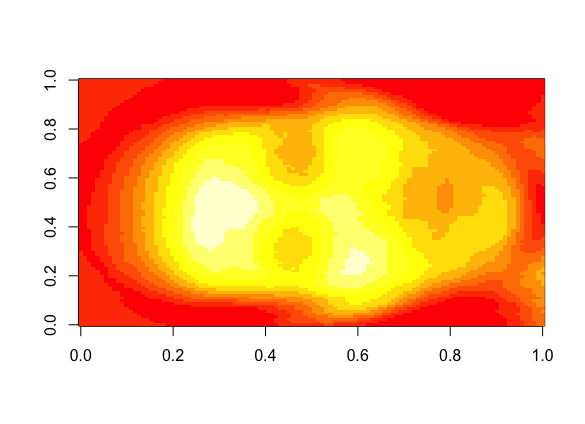
\includegraphics[width=0.5\textwidth]{average}
\end{figure}

The following function returns the PCA basis of size M as specified. I added a default parameter which also allows access to the eigenvalues associated with each vector of the eigenbasis.

\begin{lstlisting}[linewidth=18.4cm,language=R]
\end{lstlisting}




\end{document}
